\documentclass[a4paper,12pt,reqno]{amsart}
\usepackage{macros_M43}

\begin{document}

% ===================================================================
\hautdepage{Fiche 4\up{bis}: Vecteurs aléatoires discrets}
% ===================================================================


%-----------------------------------
\begin{exo}

  Soient $X$ et $Y$ deux variables aléatoires discrètes indépendantes et de même loi uniforme sur $\iintv{1,N}$, où $N\ge 2$ est un entier fixé. On définit les variables aléatoires $\min(X,Y)$ et $\max(X,Y)$ par:
  $
    \forall \omega\in\Omega, \quad
    \max(X,Y)(\omega)= \max\big(X(\omega),Y(\omega)\big),\quad
    \min(X,Y)(\omega)= \min\big(X(\omega),Y(\omega)\big).
  $
  \begin{enumerate}
    \item Expliquer pourquoi $\max(X,Y)\neq X$ et $\max(X,Y)\neq Y$.
    \item Montrer que le vecteur aléatoire $(X,Y)$ suit la loi uniforme sur $\iintv{1,N}^2$, c'est-à dire que tous les éléments de cet ensemble \emph{fini} ont la même probabilité d'être atteints par le vecteur aléatoire $(X,Y)$.
    \item Déterminer la loi du vecteur aléatoire $\big(\min(X,Y),\,\max(X,Y)\,\big)$.
    \item Les variables aléatoires $\min(X,Y)$ et $\max(X,Y)$ sont-elles indépendantes ?
  \end{enumerate}

\end{exo}


%-----------------------------------
\begin{exo}

  Soient $X$ et $Y$ deux variables aléatoires indépendantes de même loi géométrique de paramètre $p\in]0,1[$. Calculer $P(X\neq Y)$.

\end{exo}


%-----------------------------------
\begin{exo}

  Soient $X_1,\dots, X_n$ des variables aléatoires indépendantes et de même loi de fonction de répartition $F$ et de fonction de survie $G=1-F$.

  \begin{enumerate}
    \item Exprimer en fonction de $F$ la fonction de répartition de $\max(X_1,\dots,X_n)$.
    \item Exprimer en fonction de $G$ la fonction de survie de $\min(X_1,\dots,X_n)$.
  \end{enumerate}

\end{exo}


%-----------------------------------
\begin{exo} \emph{(La solitude du gardien de but)}

  On considère une suite de $n$ épreuves répétées indépendantes avec pour chaque épreuve trois issues possibles~: \emph{succès} avec probabilité $p$, \emph{échec} avec probabilité $q$ ou \emph{nul} avec probabilité $r$ ($p+q+r=1$). On notera respectivement $S_i$, $E_i$ et $N_i$ les événements \emph{succès}, \emph{échec}, \emph{nul} à la $i$-ème épreuve.

  \begin{enumerate}
    \item Dans cette question, $n=5$. Quelle est la probabilité d'obtenir dans cet ordre $2$ succès suivis d'un échec et de $2$ nuls~? Quelle est celle d'obtenir (sans condition d'ordre) $2$ succès, $1$ échec et $2$ nuls?
    \item Généraliser en montrant que la probabilité d'obtenir au cours des $n$ épreuves (et sans condition d'ordre) $i$ succès, $j$ échecs et $k$ nuls ($i+j+k=n$) vaut:
    $$
      \frac{n!}{i!\,j!\,k!}p^iq^jr^k.
    $$
    \item On revient au cas $n=5$ et on note $X_\ell$ la variable aléatoire codant le résultat de la $\ell$-ième épreuve par $X_\ell=1$ pour un succès, $X_\ell=-1$ pour un échec et $X_\ell=0$ pour un nul. On définit la variable aléatoire
    $$
      Z=\sum_{\ell=1}^5 X_{\ell}.
    $$
    Calculer $P(Z=0)$.
    \item \emph{Application}~: Un match de coupe entre deux équipes de football s'étant terminé sur un score nul, l'équipe qualifiée est désignée par la séance des tirs au but. Un joueur de l'équipe $A$ tire face au gardien de l'équipe $B$, puis un joueur de l'équipe $B$ tire face à celui de l'équipe $A$ et ainsi de suite jusqu'à ce que chaque équipe ait effectués $5$ tirs au but. On admet que la probabilité de réussir un tir au but est dans chaque cas de $0,7$ et que tous les tirs sont indépendants. Calculer la probabilité que les deux équipes soient encore à égalité après avoir effectué chacune ses $5$ tirs. Si une équipe a marqué plus de buts que l'autre lors de cette séance, elle est qualifiée, sinon on recommence l'épreuve avec d'autres joueurs. Calculer la probabilité de qualification de $A$ au bout de ses $5$ tirs.

    N.~B.: \emph{Il s'agit d'une modélisation légèrement simplifiée, en réalité la séance de tirs peut s'arrêter dès qu'une équipe ne peut plus être rejointe, par exemple si $A$ réussit ses $3$ premiers tirs et si $B$ les rate, il est inutile d'effectuer les deux derniers tirs.}
  \end{enumerate}

\end{exo}


%-----------------------------------
\begin{exo}

  \begin{minipage}{.77\linewidth}
  Dans tout cet exercice, le vecteur aléatoire discret $(X,Y)$ a pour support $S$ l'ensemble des six points représentés sur la figure ci-contre.
  La loi de $(X,Y)$ est donc donnée par les $P\big((X,Y)=(i,j)\big)$, pour $(i,j)\in S$.
  \end{minipage}%
  \begin{minipage}{.21\linewidth}
    \hfill
    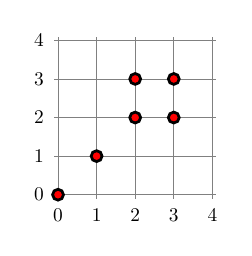
\begin{tikzpicture}[outer sep=4pt,scale=.49]
      \draw[help lines] (-.1,-.1) grid (4.1,4.1);
      \foreach ~ in {0,...,4}{
        \node[below,scale=.7] at (~,0) {~};
        \node[left,scale=.7] at (0,~) {~};
      }
      \foreach \x/\y in {0/0,1/1,2/2,2/3,3/2,3/3}
        \filldraw[fill=red, line width=1pt] (\x,\y) circle(4pt);
    \end{tikzpicture}
  \end{minipage}
    \begin{enumerate}
      \item Quelles probabilités faut-il attribuer aux différents points de $S$ pour satisfaire simultanément aux deux conditions suivantes~:
      \begin{enumerate}
        \item\label{conda} les points de $\iintv{2,3}^2$ ont tous même probabilité,
        \item\label{condb} $X$ et $Y$ suivent la loi uniforme sur $\iintv{0,3}$ ?
      \end{enumerate}
      \item Lorsque $(X,Y)$ suit la loi déterminée à la question précédente, $X$ et $Y$ sont-elles indépendantes ? On peut répondre sans calcul.
      \item Montrer qu'il existe une infinité de lois de $(X,Y)$ avec support $S$ telles que \ref{condb} soit vérifiée et $X$ et $Y$ non indépendantes.
    \end{enumerate}

\end{exo}

\end{document}

